\documentclass[11pt,a4paper]{article}

\usepackage[utf8]{inputenc}
\usepackage[T1]{fontenc}
\usepackage[a4paper,margin=1in]{geometry}
\usepackage{graphicx}
\usepackage{booktabs}
\usepackage{tabularx}
\usepackage{array}
\usepackage{enumitem}
\usepackage{etoolbox}
\usepackage{placeins}
\usepackage[numbers,sort&compress]{natbib}
\usepackage{ragged2e}
\usepackage{hyperref}
\usepackage{xcolor}

\hypersetup{
    colorlinks=true,
    linkcolor=black,
    citecolor=black,
    urlcolor=blue!50!black,
    pdftitle={MINDb Project Report},
    pdfauthor={},
}

\setlength{\parskip}{0.65em}
\setlength{\parindent}{0pt}
\renewcommand{\arraystretch}{1.15}
\setlength{\bibsep}{0pt plus 0.2ex}
\widowpenalty=10000
\clubpenalty=10000
\displaywidowpenalty=10000

\makeatletter
\newcommand{\NeedSubsectionSpace}[1]{%
    \par
    \begingroup
    \dimen@=#1\relax
    \dimen@ii=\pagegoal
    \advance\dimen@ii by -\pagetotal
    \ifdim \dimen@>\dimen@ii
        \vfil\break
    \fi
    \endgroup
}
\makeatother

\pretocmd{\section}{\NeedSubsectionSpace{12\baselineskip}}{}{}
\pretocmd{\subsection}{\NeedSubsectionSpace{10\baselineskip}}{}{}

\definecolor{reportaccent}{HTML}{184E5B}
\definecolor{reportmuted}{HTML}{5A6570}

\newcommand{\projectname}{MINDb}
\newcommand{\reporttitle}{Microbiome Interaction Network Database}
\newcommand{\reportsubtitle}{A structured platform for microbiome literature curation, exploration, and taxonomy-aware evidence integration}
\newcommand{\reportauthor}{Rafael Correia}
\newcommand{\reportprogramme}{Innovhealth 2nd Edition}
\newcommand{\reportsupervisor}{Clara Pereira}
\newcommand{\reportinstitution}{RISE-Health, Center for Translational Health and Medical Biotechnology Research}
\newsavebox{\reportabstractbox}
\newcommand{\placeholderfigure}[2]{%
    \fbox{%
        \parbox[c][#1][c]{0.9\linewidth}{%
            \centering
            \textbf{Figure placeholder}\\[0.5em]
            #2
        }%
    }%
}

\newenvironment{reportabstract}{%
    \begin{center}
    \begin{lrbox}{\reportabstractbox}
        \begin{minipage}{0.86\textwidth}
        \centering{\normalsize\bfseries\color{reportaccent}Abstract\par}
        \vspace{0.75em}
        \small
        \justifying
}{%
        \end{minipage}%
    \end{lrbox}
    \setlength{\fboxsep}{14pt}%
    \setlength{\fboxrule}{0.8pt}%
    \noindent\fcolorbox{reportaccent!30}{reportaccent!3}{\usebox{\reportabstractbox}}%
    \end{center}
}

\newcommand{\makereporttitle}{%
    \thispagestyle{empty}
    \begin{center}
        \vspace*{0.05\textheight}

        {\Large\textsc{\projectname}\par}
        \vspace{0.9em}
        {\Huge\bfseries \reporttitle\par}
        \vspace{0.7em}
        {\large\color{reportmuted}\parbox{0.84\textwidth}{\centering \reportsubtitle}\par}

        \vspace{1.5em}
        {\color{reportaccent}\rule{0.34\textwidth}{1.1pt}\par}
        \vspace{1.2em}
        \begin{minipage}[t]{0.38\textwidth}
            \centering
            {\small\textsc{Author}\par}
            \vspace{0.35em}
            {\Large \reportauthor\par}
        \end{minipage}
        \hspace{0.05\textwidth}
        \begin{minipage}[t]{0.38\textwidth}
            \centering
            {\small\textsc{Supervision}\par}
            \vspace{0.35em}
            {\Large\bfseries \reportsupervisor\par}
        \end{minipage}

        \vspace{1.5em}
        {\small\color{reportmuted}
        \begin{minipage}{0.72\textwidth}
            \centering
            {\textsc{Programme}\\[0.25em]}
            \reportprogramme\\[0.75em]
            {\textsc{Institution}\\[0.25em]}
            \parbox{0.86\linewidth}{\centering \reportinstitution}\par
        \end{minipage}\par
        }
    \end{center}
    \vspace{0.8em}
}

\begin{document}

\makereporttitle

\begin{reportabstract}
\projectname{} is a Django-based platform for curating and exploring microbiome findings reported across the scientific literature. The project was motivated by a practical problem: microbiome evidence is distributed across many papers and is difficult to compare because studies differ in cohort definitions, metadata quality, taxonomic naming, and reporting style. Instead of storing only paper-level notes or flat organism lists, \projectname{} models study context explicitly through studies, groups, comparisons, taxa, and finding records. This makes it possible to preserve how evidence was reported while still supporting structured querying and exploration.

The implemented system combines a PostgreSQL database, a server-rendered web interface, an admin-oriented import workflow, and a taxonomy support component called Taxon Bridge. Qualitative findings such as enriched or depleted taxa are stored alongside quantitative per-group measurements when available, and optional diversity metrics can also be represented. The result is an early but functional prototype that provides a solid foundation for centralized microbiome evidence integration, reproducible curation, and future graph-based analysis.
\end{reportabstract}

\section{Introduction}

The human microbiome has become an important topic in biomedical and bioinformatics research because microbial communities are increasingly linked to health, disease, treatment response, and environmental exposure \citep{lynch2016human}. A large number of microbiome studies now report associations between specific taxa and disease states, as well as broader community-level trends such as altered diversity or shifts in composition. At the same time, even healthy individuals show substantial microbiome variation across body sites and between subjects, which already makes interpretation and comparison non-trivial before methodological differences are considered \citep{hmp2012structure}. Recent work also continues to emphasize that microbiome data, metadata, and analysis workflows remain difficult to share, compare, and reuse consistently across studies \citep{huttenhower2023sharing,zass2024toolkit}.

This project addresses that problem through \projectname{}, the Microbiome Interaction Network Database. The aim of the platform is not simply to archive papers, but to curate literature-derived evidence in a form that is structured enough to support later querying, comparison, and visualization. In particular, the project is designed to preserve study context rather than collapsing findings into decontextualized organism lists. A taxon reported as increased in one subgroup versus another should remain attached to the comparison that produced that statement. This general need for structured cross-study comparison has also been recognized by recent community curation efforts for microbiome differential-abundance signatures \citep{geistlinger2024bugsigdb}.

The core goals of the project were therefore to:

\begin{itemize}[leftmargin=1.5em]
    \item centralize microbiome literature evidence in one curated platform;
    \item represent studies, cohorts, comparisons, taxa, and findings explicitly;
    \item support both qualitative and quantitative evidence;
    \item improve reproducibility by keeping import provenance and structured records;
    \item provide a web interface for browsing and exploration; and
    \item establish a practical foundation for later meta-analysis and network-based interpretation.
\end{itemize}

The current system should be understood as an early but working prototype. The priority was to build a correct and extensible structure for curation and exploration, rather than a fully polished production system. In practice, that meant focusing on a dependable data model, a clear import path, and browseable interfaces that already demonstrate the value of structured evidence capture.

The intended audience for the platform is also broader than one-off internal note taking. A resource such as \projectname{} can support the work of students, curators, and researchers who need to revisit the literature repeatedly, inspect how a finding was contextualized in a paper, and compare evidence across studies without reconstructing the same spreadsheet logic each time. It is also meant to support later reuse through filtering, graph-based exploration, and provenance-aware review of imported findings. This practical reuse case strongly influenced the emphasis on explicit relationships and browseable records.

The rest of this report follows that same progression from problem to implementation. It first motivates the need for structured microbiome curation, then describes the data model, the implementation architecture, the taxonomy support workflow, the web interface, and the main limitations that remain in the current prototype.

\section{Background and Motivation}

\subsection{Challenges in comparing microbiome studies}

Microbiome studies are heterogeneous in several ways. Different papers may define disease groups differently, use different controls, recruit from different cohorts, or report multiple subgroups within the same publication. Metadata quality is also inconsistent. Some studies clearly describe age, geography, cohort source, or sequencing details, while others report only a subset of that information. Even when papers investigate similar diseases, the comparison being made may not be equivalent. These issues have been serious enough that dedicated reporting guidelines, metadata toolkits, and curated comparison resources have been proposed to improve consistency and reproducibility across the field \citep{mirzayi2021storms,geistlinger2024bugsigdb,zass2024toolkit}. More generally, biomedical informatics research on disease ontologies continues to emphasize that inconsistent disease terminology and coding practices make cross-resource integration difficult unless they are harmonized into a computable common framework \citep{vasilevsky2025mondo}.

Taxonomic reporting creates an additional challenge. Organisms may be reported using outdated names, synonyms, abbreviated labels, inconsistent capitalization, or different taxonomic ranks. One paper may report a genus while another reports a species within that genus. This makes direct aggregation difficult unless taxonomy is handled carefully. More broadly, the development of standards such as MIxS reflects the long-standing need for more structured and interoperable microbiome metadata and sample descriptions \citep{yilmaz2011mixs}.

Finally, results are not always reported numerically. Many microbiome papers summarize findings as directional statements such as ``enriched in disease'', ``depleted in controls'', or ``increased relative abundance'', without publishing a consistent machine-readable table of values. STORMS was proposed in part because incomplete and inconsistent reporting makes microbiome studies harder to interpret and compare \citep{mirzayi2021storms}. More recent benchmarking work also shows that even downstream microbiome differential-abundance analysis still lacks methodological consensus, and that confounding and method choice can materially affect reproducibility and inferred biological conclusions \citep{wirbel2024benchmark,pelto2025elementary}. A useful platform therefore needs to represent both exact measurements and qualitative evidence.

\subsection{Need for structured curation}

Spreadsheets remain useful for manual curation, but they become limiting once the goal is systematic reuse. They do not naturally enforce relationships between records, reliable uniqueness constraints, or rich navigation across studies, groups, taxa, and findings. They also make provenance harder to track across repeated imports, edits, and revisions.

A structured database offers clear advantages. It can preserve relationships explicitly, validate inputs, prevent inconsistent duplication, and support queries that would otherwise be cumbersome. Examples include finding taxa reported as depleted in a disease-related comparison, listing all groups belonging to a paper, or reviewing findings imported from one batch. This matters in a domain where small modeling mistakes can distort scientific interpretation.

Recent microbiome-signature databases show that standardized curation makes findings easier to compare across conditions, body sites, and studies \citep{geistlinger2024bugsigdb}. At the same time, reviews of microbiome data sharing and metadata practice still argue that stronger standardization is needed for genuine interoperability and reuse \citep{huttenhower2023sharing,zass2024toolkit}. \projectname{} follows the same logic while preserving explicit study, group, comparison, and provenance context in a relational platform.

\subsection{Importance of comparison context}

A central design decision in \projectname{} is to preserve comparison context. A directional microbiome statement is incomplete if it is detached from the groups being compared. For example, the meaning of ``increased \textit{Bacteroides}'' depends on whether the comparison was disease versus healthy control, severe disease versus mild disease, or one cohort versus another.

For this reason, the platform does not flatten the literature into simple taxon lists. Instead, it stores comparisons as first-class records and attaches qualitative findings to those comparisons. Quantitative values are linked to individual groups, because abundance values are properties of one group rather than a relationship between two taxa. This modeling choice is fundamental to the usefulness of the database.

\subsection{Derived system requirements}

Once these problems are stated clearly, they lead directly to a set of technical requirements. The platform must support structured records rather than free text alone, preserve publication and cohort context, tolerate incomplete reporting, and keep enough flexibility to store heterogeneous metadata without making the schema unmanageably large. It must also support a cautious curation workflow because imported literature data can contain ambiguity, especially in taxon naming.

These requirements explain why the project combines a compact relational model with validation, provenance tracking, and taxonomy-aware resolution. In other words, the design is not only a software choice but a direct response to the shape of the source material.

\section{Data Model and Design Logic}

\subsection{Core entities}

The conceptual model of \projectname{} revolves around a small set of linked entities that capture the structure of literature-derived evidence. The main entities are study records, study groups, comparisons, taxa, and findings. This keeps the design compact while still retaining the context needed for later analysis.

\begin{table}[htbp]
    \centering
    \small
    \caption{Main data entities in \projectname{} and their roles.}
    \label{tab:entities}
    \begin{tabularx}{0.98\linewidth}{>{\raggedright\arraybackslash}p{3.8cm} >{\raggedright\arraybackslash}X}
        \toprule
        \textbf{Entity} & \textbf{Role in the platform} \\
        \midrule
        Studies & Publication-level records with bibliographic context such as title, DOI, journal, year, and notes. \\
        Groups & Study arms, cohorts, subgroups, or other analytical populations within a study. \\
        Comparisons & Explicit directional contrasts between two groups. \\
        Taxa & Canonical microbial entities used throughout the database. \\
        Qualitative findings & Direction-of-change evidence for one taxon in one comparison, such as enriched, depleted, increased, or decreased. \\
        Quantitative findings & Numeric values for one taxon in one group, for example relative abundance measurements. \\
        Metadata variables and values & Lightweight structured metadata for groups without overloading the main schema with many sparse columns. \\
        Import batches & Provenance records describing validation status and import outcomes. \\
        Diversity metrics & Optional alpha- and beta-diversity measurements when these are available. \\
        \bottomrule
    \end{tabularx}
\end{table}

This structure reflects the reality of microbiome curation. Papers contain multiple groups, groups participate in comparisons, and findings emerge from those comparisons or from measurements observed within those groups. The schema is therefore designed to mirror the logic of the evidence rather than forcing it into a simpler but less accurate layout.

\subsection{Schema design principles}

Several design principles guided the model. First, common and analytically important concepts are stored as explicit tables rather than hidden inside generic metadata fields. This is why studies, groups, comparisons, taxa, and findings remain first-class records. Second, the schema keeps the direct columns focused on information that is consistently useful, while sparse or variable study annotations can be handled through a lightweight metadata layer. Third, provenance is treated as part of the data model rather than as an afterthought, because imported evidence may need to be traced back to a particular curation batch.

Another important principle is that the schema should support browsing as well as storage. It is not enough to create a technically valid set of tables if the resulting records are difficult to inspect or explain. The current model was therefore shaped with list views, detail views, admin editing, and future graph serialization in mind.

\subsection{Qualitative and quantitative evidence}

The platform distinguishes between two major types of evidence. Qualitative findings capture direction-of-change statements such as enriched, depleted, increased, or decreased. These are common in microbiome papers and are often the only practically extractable outcome from narrative or table-based reporting. In \projectname{}, a qualitative finding is always tied to a comparison because the statement only makes sense relative to the two groups being contrasted.

Quantitative findings capture numeric values for one taxon in one group. This may include relative abundance values or similar per-group measures when they are explicitly reported. This design avoids an older but misleading idea of modeling abundance as a relationship between organism A and organism B. In practice, abundance is a property of a taxon within a group.

Together, these two evidence types allow the system to store both coarse and fine-grained information. Even when exact values are unavailable, the platform can still capture the reported biological direction. When values are available, they can be stored in a way that remains consistent with the broader data model.

\subsection{Explicit comparisons as core units}

Comparisons are central because they capture the analytical claim being made by a study. In many papers, the biologically meaningful result is not ``this taxon exists'' but ``this taxon differs between these two groups''. By representing the comparison explicitly, \projectname{} makes later querying more meaningful. It becomes possible to ask which taxa are repeatedly reported as enriched in disease-related groups, how evidence changes when comparing severe versus mild cases rather than disease versus control, and to aggregate directional findings into disease--taxon or comparison--taxon networks without losing sight of where the evidence came from.

\subsection{Taxonomy-aware representation}

Taxonomy handling is an important extension of the core model. The implemented platform uses canonical taxon records together with taxon names and a closure table for lineage traversal. This allows the system to keep one normalized taxonomic representation while still remembering alternate names and supporting lineage-aware filtering.

This matters because literature findings are often reported at mixed ranks. A user may want to browse evidence at the leaf level, or instead group results by genus, family, or phylum. A taxonomy-aware representation makes that possible without rewriting the underlying curated data.

\subsection{Data integrity and provenance}

The conceptual model also depends on integrity rules. Studies should not duplicate the same DOI unnecessarily, groups should be unique within a study, and comparisons should connect distinct groups that belong to the correct study. Similarly, qualitative findings and quantitative findings should remain unique at the level of their main identifying context. These constraints are important because curated literature data can easily accumulate accidental duplicates when multiple import rounds or manual edits take place.

Provenance is equally important. By linking imported records to an import batch, the platform preserves a trace of how data entered the system. This supports review, debugging, and later refinement of the curation process. In a scientific database, knowing where a record came from is part of making it trustworthy.

\section{Implementation}

\subsection{Technology stack}

The implemented prototype uses Django as the web framework and PostgreSQL as the underlying relational database. This combination was chosen because it provides strong support for structured models, migrations, validation, and admin-based data management while remaining practical for a student-scale project. Bootstrap is used for the frontend interface so that the site remains readable and responsive without introducing heavy client-side complexity.

For graph logic, the project uses Python-based network construction and a browser rendering layer. The graph-related processing is handled on the backend, while the resulting node and edge data are delivered to the frontend for interactive display. This keeps the data logic close to the database and avoids the need for a separate analytics service.

\begin{table}[htbp]
    \centering
    \small
    \caption{Main implementation components and their roles in the current prototype.}
    \label{tab:stack}
    \begin{tabularx}{0.98\linewidth}{>{\raggedright\arraybackslash}p{3.6cm} >{\raggedright\arraybackslash}X}
        \toprule
        \textbf{Component} & \textbf{Role} \\
        \midrule
        Web framework (Django) & Routing, ORM access, forms, admin integration, and server-rendered views. \\
        Database (PostgreSQL) & Persistent storage for curated studies, comparisons, taxa, findings, metadata, and provenance. \\
        Interface layer (Bootstrap) & Responsive presentation for the public site and browser pages. \\
        Admin interface & Manual curation environment for staff users and schema-aware record editing. \\
        Import services & Preview-first parsing, validation, duplicate checks, and batch execution for CSV and workbook ingestion. \\
        Taxonomy support (Taxon Bridge) & Name resolution and lineage-aware taxonomic support during preview and import. \\
        Graph services & Backend construction of lineage-aware qualitative graph payloads for interactive exploration. \\
        \bottomrule
    \end{tabularx}
\end{table}

\subsection{Application structure}

The current implementation is organized around a few focused Django apps. The database layer defines the core models for studies, groups, comparisons, taxa, findings, metadata, and import provenance. The browser layer provides server-rendered list and detail pages with searching, filtering, sorting, and pagination. The core web layer provides the homepage, staff workspace, and graph view. A dedicated import layer handles upload, validation, preview, and confirm steps for both contract CSV files and a curator workbook.

This structure is intentionally conservative. The goal was not to build a complex single-page application, but a maintainable system whose behavior remains easy to inspect. Server-rendered pages are well suited to a curation platform because they are simple, stable, and fit well with Django's built-in strengths.

This choice also helps with long-term maintainability. For a data-centric project, complexity in the frontend can easily exceed the real needs of the platform. By keeping the application largely server-rendered, the implementation effort remains focused on schema correctness, import reliability, and query behavior rather than on synchronizing large amounts of duplicated client-side state.

\subsection{Import and curation workflow}

A major practical requirement of the project was support for staged data ingestion. Literature curation is error-prone, and taxonomy resolution can be uncertain, so it is risky to write directly to the database without review. The implemented import workflow therefore follows a preview-first pattern.

Users upload either a structured CSV file or the curator Excel workbook through an admin-facing interface. The system parses the file, checks required columns, validates relationships, detects duplicates, and builds a preview of rows that are ready to import. Workbook ingestion also filters records according to paper status and resolves cross-sheet identifiers before any write occurs.

The import layer creates and updates \texttt{ImportBatch} records so that each batch has provenance and summary statistics. This is important for traceability. If a curation batch later needs to be reviewed, the system can show what was imported, from which source, and with what success or error counts.

The preview step is particularly important because it separates parsing from commitment. Curators can inspect valid rows, validation errors, and duplicates before any database write occurs. For workbook-based imports, this also allows the system to surface skipped rows and taxon-resolution issues in a transparent way. In practice, this is one of the strongest safeguards in the project because it reduces the risk of silently introducing low-quality data.

The import workflow also reflects a pragmatic view of curation. Not every problematic row should block an entire batch. Some issues should lead to a clear warning and a skipped record rather than a total failure. This is especially true for taxonomy-related edge cases, where the correct operational behavior may be to defer uncertain rows for later review while still importing the rest of the validated material.

\subsection{Taxonomy persistence and lineage support}

The current implementation stores taxa as canonical records and keeps additional supporting tables for names and lineage traversal. A \texttt{TaxonName} table captures synonyms, aliases, and imported-as-written names, while a closure table stores ancestor--descendant relationships. This enables branch filtering, lineage display, and rank-based rollup.

This is especially valuable for qualitative graph exploration. Findings are stored at the reported leaf taxon, but graph queries can later roll them up to a higher rank such as genus or family. In other words, the database preserves detail while still supporting more interpretable summaries.

The lineage-aware design also improves browsing. A user may wish to inspect all taxa inside one branch, review the lineage of a selected taxon, or compare evidence at different levels of taxonomic granularity. These tasks become much easier when ancestry is stored explicitly instead of reconstructed ad hoc from imported names.

\subsection{Interface and graph view}

The website exposes several user-facing views. Public pages include a homepage, a browser landing page, and list/detail views for studies, groups, comparisons, taxa, qualitative findings, and quantitative findings. These pages support standard exploration tasks such as search, filter, sort, and pagination.

In addition, the current prototype includes a graph view derived from qualitative findings. This view allows evidence to be filtered by study, direction, disease-like target group, taxon, taxonomic branch, and taxonomic rank. The graph is arranged around a simple but useful semantic layout: disease nodes in the center, taxa enriched in disease on one side, and taxa depleted in disease on the other. This design is grounded in the directional comparison model rather than in abstract co-occurrence alone.

Although visually simple, this graph view demonstrates one of the broader goals of the project: database structure should enable multiple forms of interpretation. The same curated records that power ordinary list and detail pages can also be serialized into a higher-level disease--taxon view. This is a strong argument in favor of the underlying schema because it shows that explicit comparisons and finding records support both precise lookup and broader exploratory analysis.

\section{Taxon Bridge}

\subsection{Rationale for Taxon Bridge}

Taxonomy normalization is one of the most difficult parts of microbiome literature integration. Papers frequently use inconsistent naming, outdated labels, partially specified taxa, or mixed reporting levels. Without a dedicated resolution step, a database quickly accumulates duplicate or ambiguous organism entries, which reduces query quality and makes later aggregation unreliable.

Taxon Bridge was developed as a supporting tool to address this issue. Its purpose is not to replace the main platform, but to strengthen it by providing a more reliable bridge between raw names found in the literature and the canonical taxonomy-aware records stored in \projectname{}.

\subsection{Role in the workflow}

In the implemented system, Taxon Bridge is used during preview and import to help resolve taxon names and obtain lineage information. When an incoming taxon can be resolved confidently, the platform can map it to a canonical taxonomic representation and store the corresponding lineage-aware payload. When resolution is uncertain, the system flags the row for review rather than silently forcing a potentially incorrect match.

This behavior is important from a curation perspective. A microbiome evidence platform should not hide uncertainty inside the database. It is better to make ambiguous cases visible, preserve them in preview, and require a human decision when necessary.

In practical terms, this makes Taxon Bridge part of the quality-control path. It is not only a convenience layer for prettier names. It helps determine whether a literature label can be trusted as a canonical taxon, whether lineage information can be attached safely, and whether a row should move forward automatically or be held back for curator review.

\subsection{Contribution to data quality and extensibility}

Taxon Bridge improves the platform in several ways. First, it reduces name fragmentation by linking literature labels to more stable canonical taxa. Second, it enables lineage-aware filtering and grouping because taxonomic ancestry can be stored explicitly rather than inferred ad hoc later. Third, it supports future extensibility: once organism handling is normalized properly, later tasks such as cross-study comparison, taxonomic rollup, and graph summarization become much more reliable.

It is important, however, to present Taxon Bridge in proportion. The main project remains \projectname{}, the literature database and exploration platform. Taxon Bridge is an enabling component that improves organism handling, but it is not the central product of the project.

This distinction matters from a project-report perspective as well. The novelty of \projectname{} lies in the full curation and exploration workflow: the data model, the database browser, the import process, and the early graph view. Taxon Bridge strengthens one crucial part of that workflow, namely taxonomic normalization, but its value is best understood in terms of how it improves the main platform.

\section{Platform Interface}

\subsection{Public-facing views}

The public side of the platform is designed to make the curated database accessible without forcing users into the Django admin. The homepage introduces the purpose of the project and links directly to the browser and graph views. The browser landing page then presents the main record categories available for exploration.

List pages expose the main evidence types in a structured way. Studies can be browsed at paper level, groups and comparisons can be inspected to understand study design, taxa can be explored using lineage-aware filters, and findings can be searched directly. This supports both top-down exploration, such as starting from a disease or paper, and bottom-up exploration, such as starting from a taxon.

The browser is especially important because it turns the schema into something operational for users. A good data model is not very useful if the resulting records remain buried inside raw tables. By exposing records through searchable and filterable pages, the platform makes the curated content inspectable and therefore more trustworthy.

\begin{figure}[htbp]
    \centering
    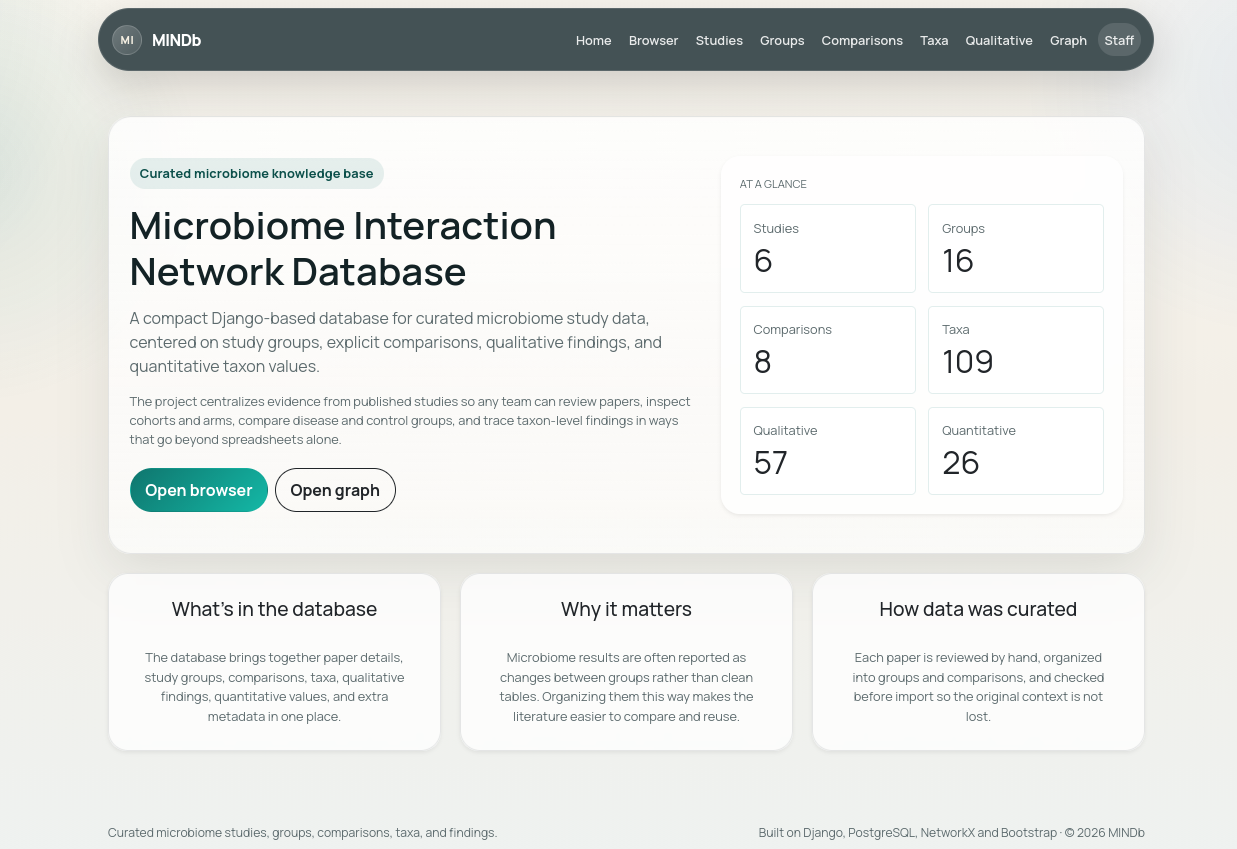
\includegraphics[width=\linewidth]{figures/mindb_homepage.png}
    \caption{Homepage of the \projectname{} platform, presenting the project purpose and linking to the browser and graph views.}
    \label{fig:homepage}
\end{figure}

\begin{figure}[htbp]
    \centering
    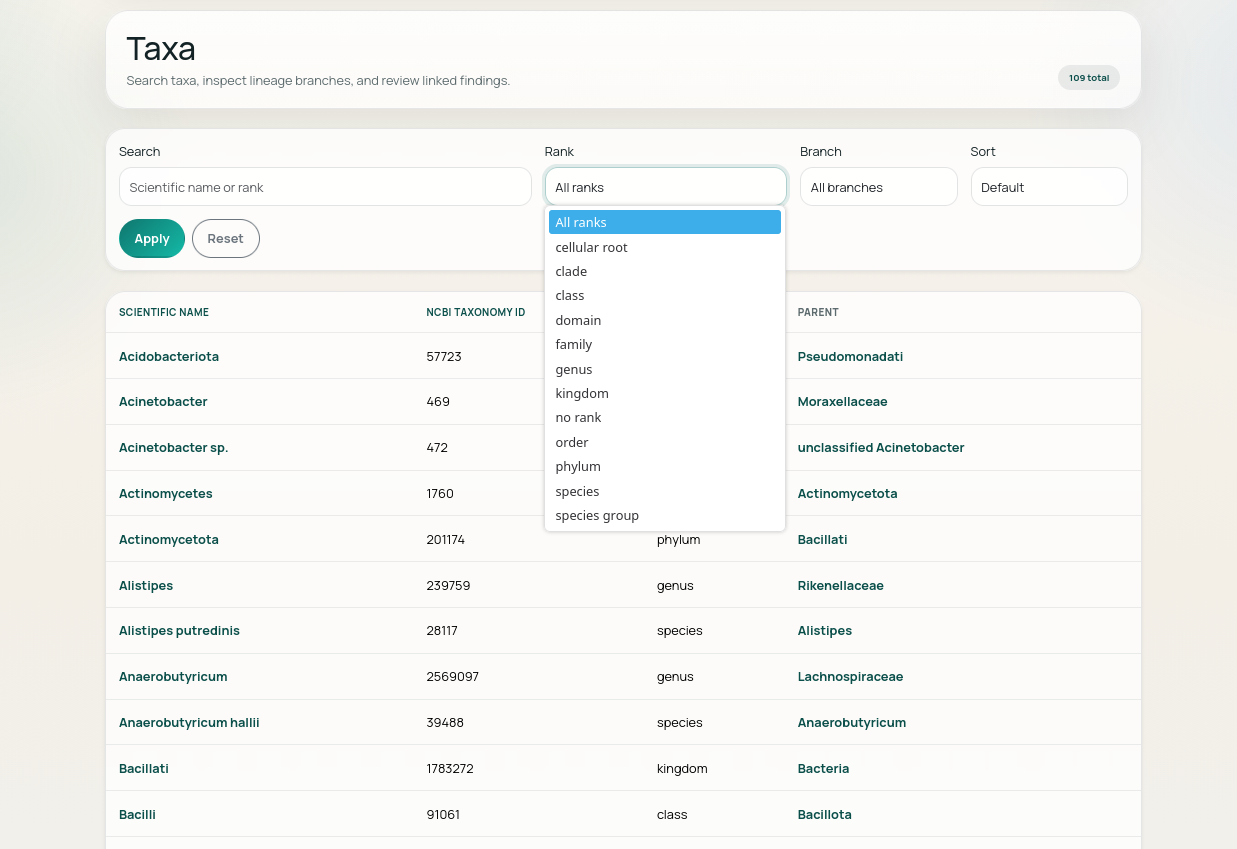
\includegraphics[width=\linewidth]{figures/mindb_browser.png}
    \caption{Example of the structured browser interface used to search, filter, sort, and inspect curated records.}
    \label{fig:browser}
\end{figure}

\subsection{Curation and administration}

The platform also includes staff-only functionality for curation and maintenance. A protected staff workspace links to import tools, the Django admin, and a generated model diagram. Through Django admin, curators can edit studies, groups, comparisons, taxa, qualitative findings, quantitative findings, metadata variables, metadata values, diversity metrics, and import batches. The admin environment also supports broader platform administration such as user management and permission-aware access control through Django's standard administrative system.

From a project perspective, this matters because literature curation is not only a viewing problem. It is also a data stewardship problem. The ability to maintain records manually, inspect schema structure, and upload new content through a validated workflow is essential to the usefulness of the platform.

The combination of manual admin editing and structured batch upload is deliberate. Some corrections are easiest to make one record at a time, especially during early prototyping or spot fixes. Other tasks, such as ingesting curated workbook content, are more efficient through batch-oriented import. Supporting both modes makes the system more realistic as a curation platform.

\begin{figure}[htbp]
    \centering
    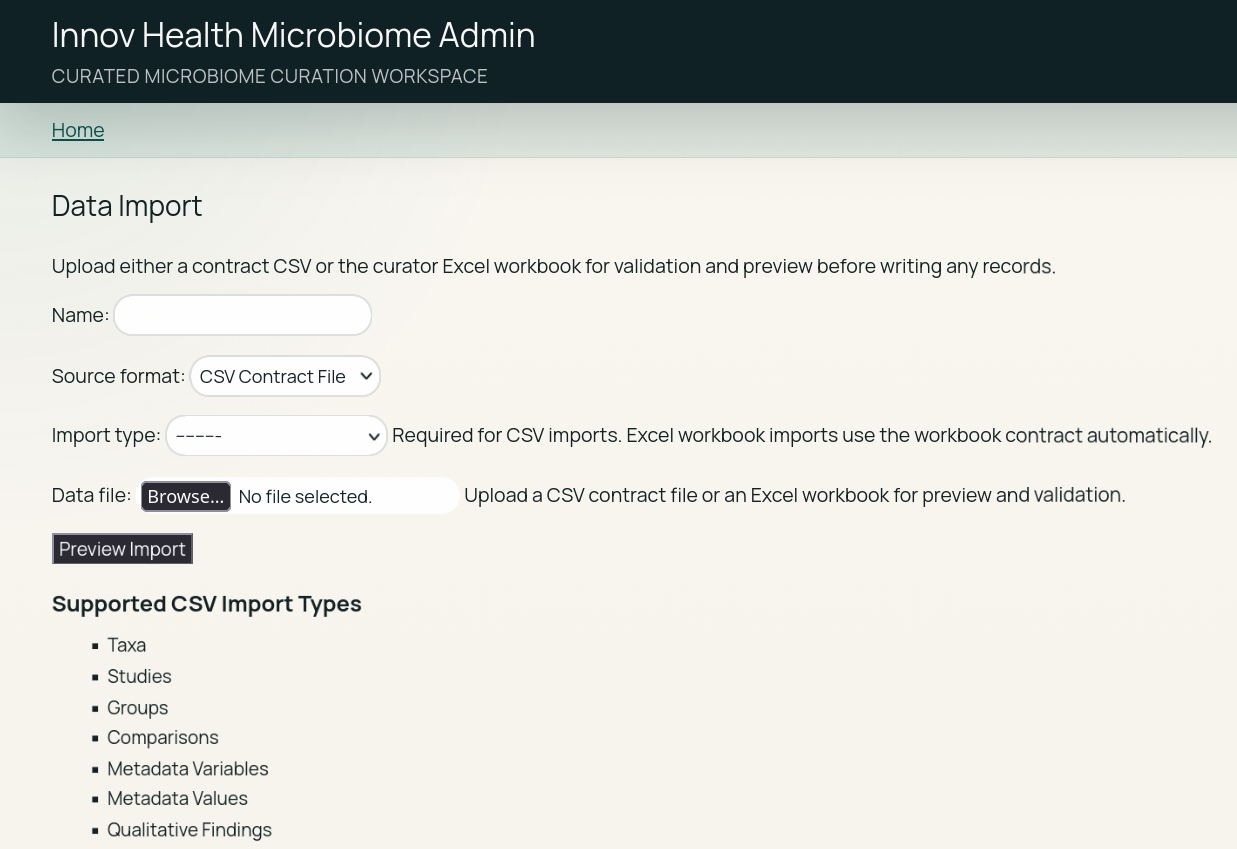
\includegraphics[width=\linewidth]{figures/minddb_admin_import.png}
    \caption{Admin-side workflow for uploading, previewing, and confirming curated data imports before records are written to the database.}
    \label{fig:adminimport}
\end{figure}

\subsection{Graph exploration}

Although the project is not centered on visualization alone, graph-based exploration is a useful extension of the curated database. The current implementation includes an interactive disease--taxon network derived from qualitative findings. Users can apply study and direction filters, constrain the graph to one taxonomic branch, and roll findings up from leaf taxa to higher ranks such as genus or family.

This view is valuable because it gives a compact overview of directional evidence without discarding the underlying database structure. It does not replace the browser; instead, it acts as a second lens over the same curated records.

This is also a useful proof of concept for future work. If qualitative findings can already be organized into a lineage-aware disease--taxon graph, then later extensions such as richer edge summaries, cross-study weighting, or comparative network views become easier to imagine and implement on the same foundation.

\begin{figure}[htbp]
    \centering
    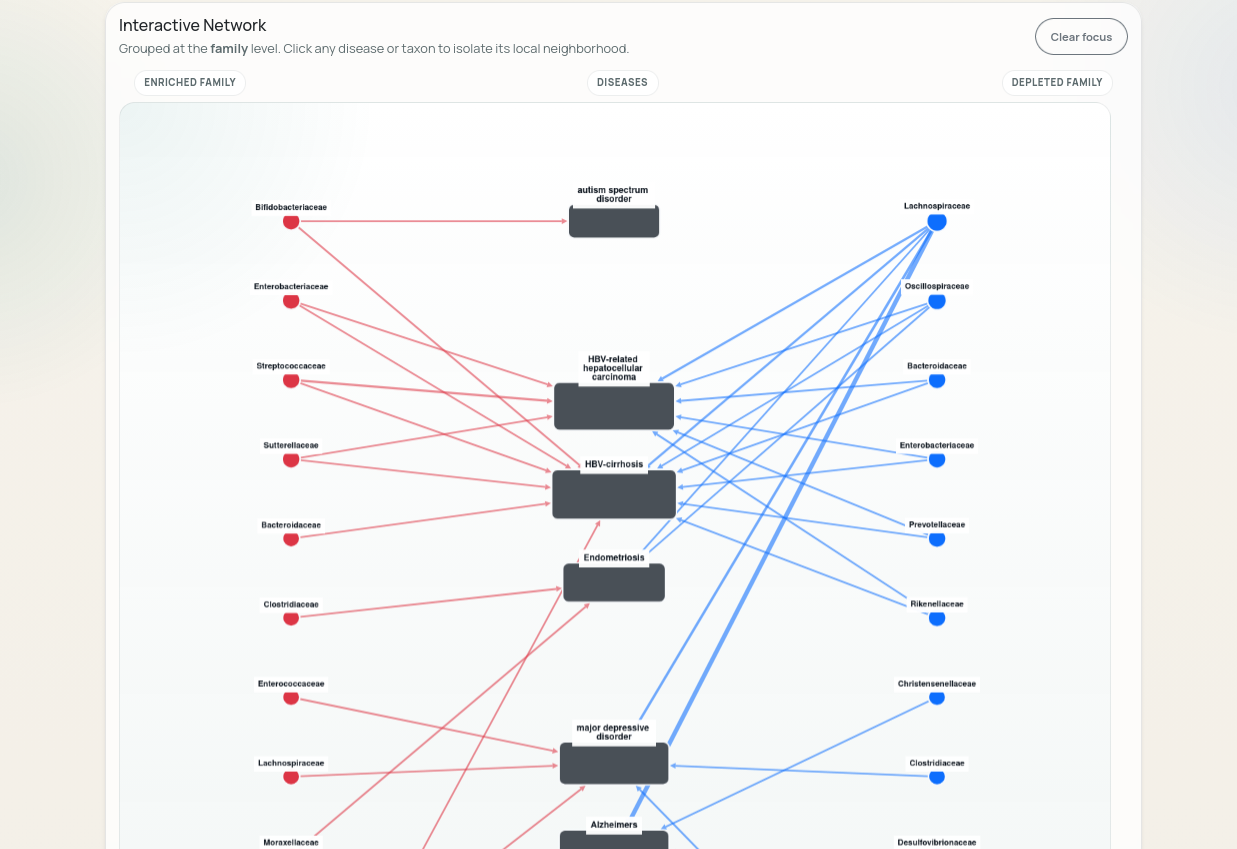
\includegraphics[width=\linewidth]{figures/minddb_graph.png}
    \caption{Interactive graph view showing qualitative disease--taxon relationships derived from curated comparison records.}
    \label{fig:graph}
\end{figure}

\subsection{Taxon Bridge workflow}

Taxon Bridge is most visible during import preview, where incoming names can be resolved, normalized, or flagged for review. This gives curators a chance to inspect organism handling before data are committed. From a usability perspective, this is preferable to either accepting raw names blindly or rejecting ambiguous rows without explanation.

\begin{figure}[htbp]
    \centering
    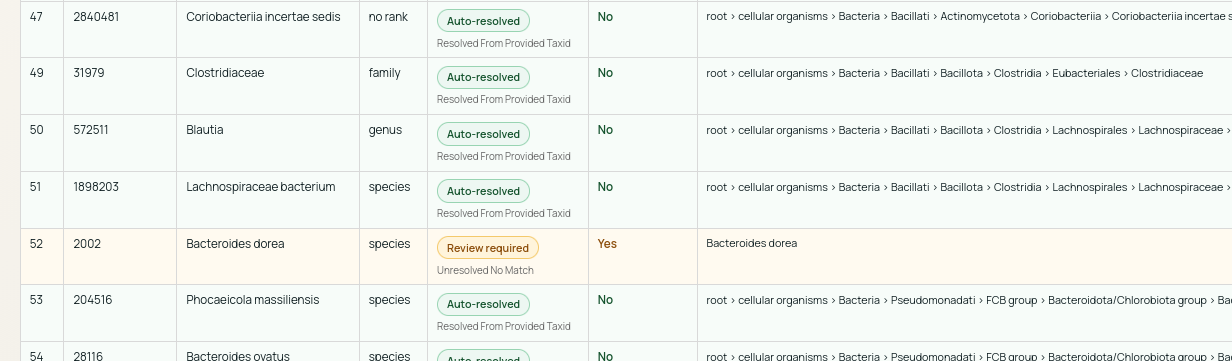
\includegraphics[width=\linewidth]{figures/taxon_bridge_preview.png}
    \caption{Taxon Bridge-assisted preview showing taxonomy-aware resolution before imported findings are committed to the database.}
    \label{fig:taxonbridge}
\end{figure}

\FloatBarrier

\section{Limitations and Future Directions}

The current platform should be described as an early-stage but functional prototype. The core ideas have been implemented: structured models, browser views, a curation workflow, taxonomy-aware handling, and a graph layer derived from qualitative findings. This is enough to demonstrate that the project concept is technically viable and that the chosen data model supports meaningful exploration.

At the same time, several limitations remain. Literature curation is still labor-intensive and requires domain-aware manual effort. Not all papers report findings in a clean or consistent form, so extraction remains partly interpretive. Metadata standardization is also challenging because published studies vary widely in what they report. Even with Taxon Bridge, taxonomy resolution is not always automatic; uncertain names still require human review, especially when papers use outdated terminology or ambiguous rank information.

The current graph layer is useful but intentionally lightweight. It is designed as an exploration view over curated findings rather than as a full network analysis suite. Likewise, the platform has been optimized more for structural correctness and maintainability than for deployment hardening, interoperability, or large-scale automation.

Another important limitation is evaluation scope. The project demonstrates architecture and workflow successfully, but it does not yet claim comprehensive literature coverage or large-scale analytical benchmarking. At this stage, the main achievement is the creation of a usable framework for curated evidence integration. Future evaluation could therefore focus not only on software robustness but also on curation consistency, breadth of database coverage, and the practical usefulness of the resulting dataset for downstream analysis.

There are also trade-offs in the decision to keep the system intentionally compact. A lightweight architecture is easier to understand and maintain, but it means that some advanced features remain outside the current scope. These include automated literature mining, richer ontology support, more complex user roles, external programmatic APIs, and deeper analytical dashboards. None of these are impossible within the current direction, but they were not prioritized over the more fundamental problem of correct data representation.

Natural directions for future work include:

\begin{itemize}[leftmargin=1.5em]
    \item broader literature coverage and larger curated datasets;
    \item richer metadata normalization and controlled vocabularies;
    \item a disease-standardization layer, analogous to Taxon Bridge, to normalize disease names, subgroup labels, and related controlled vocabulary across curated studies, potentially drawing on ontology harmonization efforts such as Mondo \citep{vasilevsky2025mondo};
    \item more automated assistance for extraction and import preparation;
    \item tighter taxonomy integration and continued improvement of resolution workflows;
    \item additional graph summaries and comparative analysis features; and
    \item stronger deployment, testing, and user-facing polish.
\end{itemize}

These are meaningful next steps, but they depend on the same foundation established here: a clear and defensible representation of studies, groups, comparisons, taxa, and findings.

\section{Conclusion}

\projectname{} was developed to address a clear need in microbiome informatics: the need to centralize literature-derived evidence in a form that preserves study context and remains usable for later exploration. Rather than treating papers as isolated notes or reducing results to flat organism lists, the project models studies, groups, comparisons, taxa, and findings explicitly. This makes the platform more suitable for structured querying, reproducible curation, and future synthesis across publications.

The current implementation demonstrates that this approach is practical. A Django and PostgreSQL architecture provides a stable backbone for data management, the web interface supports browsing and exploration, the import workflow adds validation and provenance, and Taxon Bridge strengthens taxonomy-aware normalization. Although the system is still at prototype stage, it already provides a credible foundation for centralized microbiome evidence integration and future bioinformatics work built on curated literature data.


\begingroup
\small
\bibliographystyle{abbrvnat}
\bibliography{references}
\endgroup

\end{document}
